
\section{Paradigms}
\label{ParadigmsSection}

There are three general ideas that repeat throughout the max flow algorithms in the literature.


\subsection{Augmenting Paths}
The first idea was introduced by L. R. Ford and D. R. Fulkerson in 1956 \cite{FordFulkerson}, and consists of finding augmenting paths in the graph.
The basic idea is that if you repeatedly find and saturate all augmenting paths in the graph, no more flow can be sent from $s$ to $t$, and you must have a max flow.

The number of augmenting paths an algorithm finds depends on the order in which augmenting paths are found. 
For instance if you consider the graph in Figure~\ref{augmentingPathsExample}, an augmenting path can be made with minimum residual capacity $1$.
Following that path, another can be found with residual capacity $1$ if you follow the middle edge in the opposite direction.
So on this graph, anywhere from $2$ to $1000$ augmenting paths can be found.
\begin{figure}[ht!]
\centering
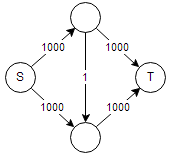
\includegraphics{augmentingPathsExample.png}
\caption{}
\label{augmentingPathsExample}
\end{figure}
If we didn't have integer capacities, graphs can be created for which infinity many augmenting paths could be found if they are found in a special order.

The idea that no more flow can be sent if no augmenting path can be found is also what is often used to prove correctness of a max flow algorithm. 
If the flow is valid, and there is no augmenting paths in the residual graph, you must have found the max flow.

The algorithm explained in Section~\ref{EK1972Section} is based on finding augmenting paths.

\subsection{Blocking Flow}

The \emph{blocking flow} idea was introduced by E. A. Dinic in 1970 \cite{dinic1970}.
The idea is to construct a \emph{layer graph} that only contains the edges that increase the distance from $s$.
The nodes in the layer graph are the same as the nodes in the graph $G$,
and an edge $(u, v)$ only exists in the layer graph if $distance(s, u) < distance(s, v)$, and $r(u, v) > 0$.
In most blocking flow algorithms, it is sufficient that the layer graph is a directed acyclic graph (DAG).
The general idea is that all paths from $s$ to $t$ have the same length, so you can find the augmenting paths shortest to longest,
but algorithms like Goldberg Rao \cite{Goldberg1998} actually might add some edges $(u, v)$ to the graph where $distance(s, u) = distance(s, v)$,
as long as the graph remains acyclic.

The interesting thing about the layer graph is that it contains all augmenting paths of a certain length $k$, where $k$ is the length of the shortest augmenting path in the residual network of $G$.
The algorithm can now find the max flow in this smaller layer graph. This flow is denoted the \emph{blocking flow}.
Most blocking flow algorithms then continue by updating the residual network of the original graph with the blocking flow, and calculating a new layer graph, which will have a bigger $k$.
This process repeats until all augmenting paths have been found.

\begin{figure}[!ht]
\centering
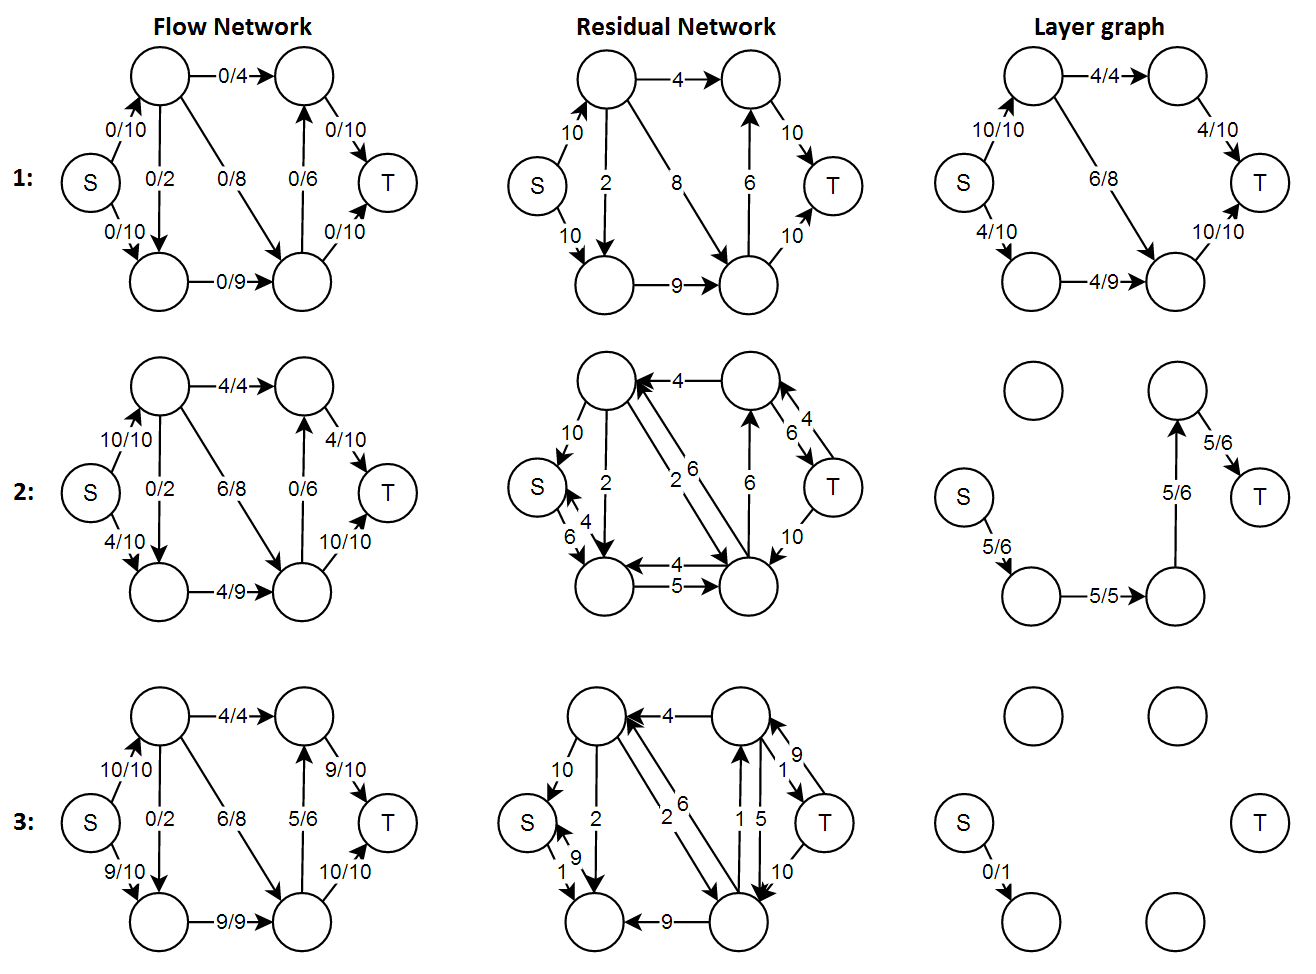
\includegraphics[width=120mm]{dinicExample.png}
\caption{An example of running a blocking flow algorithm.}
\label{dinicExample}
\end{figure}

The algorithm explained in Section~\ref{DinicSection} is an example of a blocking flow algorithm.
For an example of running a blocking flow algorithm, see Figure~\ref{dinicExample}.


\subsection{Push Relabel}

The \emph{push relabel} idea was introduced by A. V. Goldberg and R. E. Tarjan in 1988 \cite{Goldberg1988}.
This idea differs substantially from the previous two ideas, in that it does not explicitly find augmenting paths.
Instead it works by manipulating a preflow in the algorithm, by violating the flow conservation constraint throughout the algorithm, and pushing excess between individual nodes by adding flow on the edges in the graph.

The idea is to assign a non-negative integer \emph{label} $d(v)$ to each node. 
It starts with giving $s$ the label $n$, and all other nodes the label $0$. 
It then pushes as much flow as possible from $s$ to the neighbours of $s$. The main part of the algorithm is a sequence of pushes and relabels. 
A relabel on a node increases its label by at least one. 
A push sends flow from one node $u$ to another node $v$, but this is only allowed if $d(u) > d(v)$. 
Apart from in the initialization, the nodes $s$ and $t$ are never relabelled, and are never the source of a push.

A relabel should only be performed if a node has some excess, but no place to send it. 
If a node receives excess, it can always send it back to the node it received it from, so if it has no place to send its excess, there must be some neighbour with a higher label, where the excess can be sent.

What is going to happen when running a push relabel algorithm is a sequence of pushes and relabels that move excess around the graph from node to node.
At some point, the nodes will start to be relabelled above $n$. 
When this happens, $t$ is no longer reachable.
A result of having labels above $n$ is that excess will  begin to be pushed back towards $s$. 
Eventually, all the excess will have been pushed to either $s$ or $t$, which means that the flow conversation constraint is fulfilled. 
At this point, a push relabel algorithm will have found a valid flow, which is in fact the max flow.

\begin{figure}[!ht]
\centering
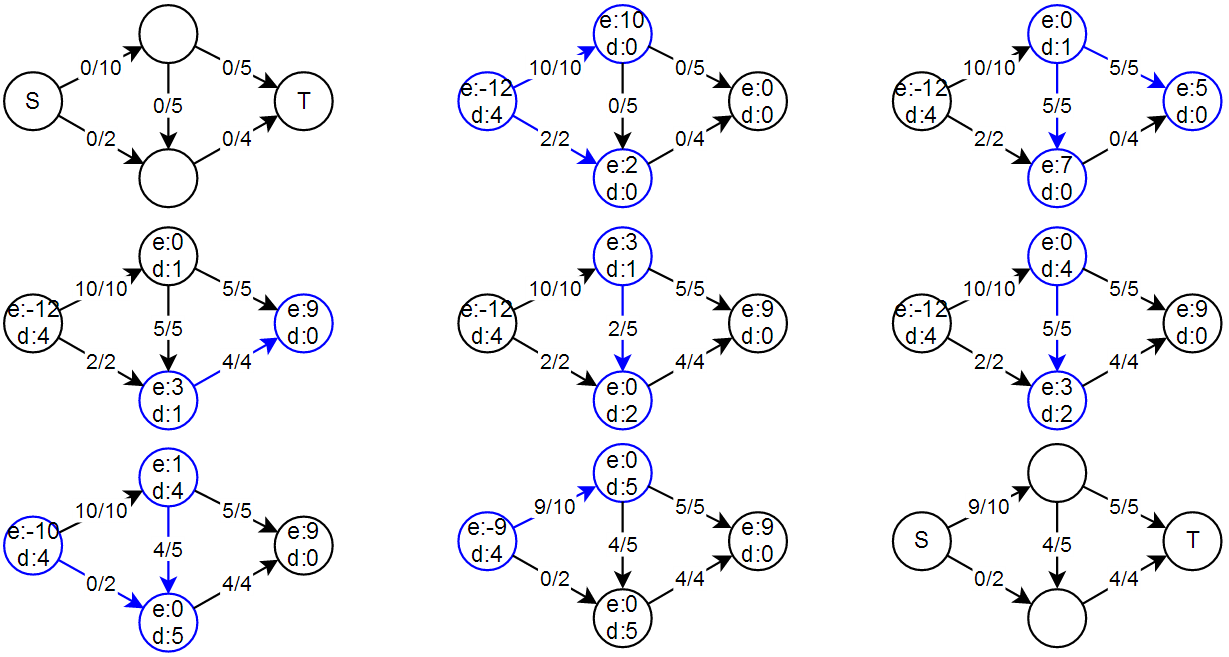
\includegraphics[width=120mm]{pushRelabelExample.png}
\caption{An example of running a push relabel algorithm.}
\label{pushRelabelExample}
\end{figure}

An example of running a push relabel algorithm can be seen in Figure~\ref{pushRelabelExample}.
See Section~\ref{GoldbergTarjanSection} for details on a concrete push relabel algorithm.